\documentclass[12pt]{standalone}
\usepackage{tikz}
\begin{document}

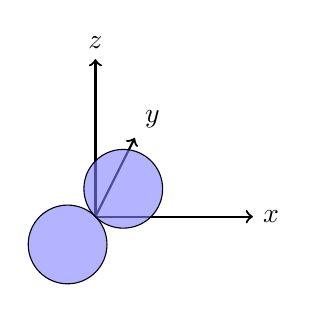
\begin{tikzpicture}

\draw[thick, ->] (0,0) -- (2,0) node[right] {$x$};
\draw[thick, ->] (0,0) -- (0,2) node[above] {$z$};
\draw[thick, ->] (0,0) -- (0.5, 1) node[above right] {$y$} ;
\filldraw[draw=black, fill = blue!50!white, fill opacity = 0.6] ({0.5/sqrt(2)}, {0.5/sqrt(2)}) circle[radius=0.5];
\filldraw[draw=black, fill = blue!50!white, fill opacity = 0.6] ({-0.5/sqrt(2)}, {-0.5/sqrt(2)}) circle[radius=0.5];

\end{tikzpicture}


\end{document}